\documentclass[journal,12pt,twocolumn]{IEEEtran}

\usepackage{setspace}
\usepackage{gensymb}

\singlespacing


\usepackage[cmex10]{amsmath}

\usepackage{amsthm}

\usepackage{mathrsfs}
\usepackage{txfonts}
\usepackage{stfloats}
\usepackage{bm}
\usepackage{cite}
\usepackage{cases}
\usepackage{subfig}

\usepackage{longtable}
\usepackage{multirow}

\usepackage{enumitem}
\usepackage{mathtools}
\usepackage{steinmetz}
\usepackage{tikz}
\usepackage{circuitikz}
\usepackage{verbatim}
\usepackage{tfrupee}
\usepackage[breaklinks=true]{hyperref}
\usepackage{graphicx}
\usepackage{tkz-euclide}
\usepackage{float}

\usetikzlibrary{calc,math}
\usepackage{listings}
    \usepackage{color}                                            %%
    \usepackage{array}                                            %%
    \usepackage{longtable}                                        %%
    \usepackage{calc}                                             %%
    \usepackage{multirow}                                         %%
    \usepackage{hhline}                                           %%
    \usepackage{ifthen}                                           %%
    \usepackage{lscape}     
\usepackage{multicol}
\usepackage{chngcntr}

\DeclareMathOperator*{\Res}{Res}

\renewcommand\thesection{\arabic{section}}
\renewcommand\thesubsection{\thesection.\arabic{subsection}}
\renewcommand\thesubsubsection{\thesubsection.\arabic{subsubsection}}

\renewcommand\thesectiondis{\arabic{section}}
\renewcommand\thesubsectiondis{\thesectiondis.\arabic{subsection}}
\renewcommand\thesubsubsectiondis{\thesubsectiondis.\arabic{subsubsection}}


\hyphenation{op-tical net-works semi-conduc-tor}
\def\inputGnumericTable{}                                 %%

\lstset{
%language=C,
frame=single, 
breaklines=true,
columns=fullflexible
}
\begin{document}
\newtheorem{theorem}{Theorem}[section]
\newtheorem{problem}{Problem}
\newtheorem{proposition}{Proposition}[section]
\newtheorem{lemma}{Lemma}[section]
\newtheorem{corollary}[theorem]{Corollary}
\newtheorem{example}{Example}[section]
\newtheorem{definition}[problem]{Definition}

\newcommand{\BEQA}{\begin{eqnarray}}
\newcommand{\EEQA}{\end{eqnarray}}
\newcommand{\define}{\stackrel{\triangle}{=}}
\bibliographystyle{IEEEtran}
\providecommand{\mbf}{\mathbf}
\providecommand{\pr}[1]{\ensuremath{\Pr\left(#1\right)}}
\providecommand{\qfunc}[1]{\ensuremath{Q\left(#1\right)}}
\providecommand{\sbrak}[1]{\ensuremath{{}\left[#1\right]}}
\providecommand{\lsbrak}[1]{\ensuremath{{}\left[#1\right.}}
\providecommand{\rsbrak}[1]{\ensuremath{{}\left.#1\right]}}
\providecommand{\brak}[1]{\ensuremath{\left(#1\right)}}
\providecommand{\lbrak}[1]{\ensuremath{\left(#1\right.}}
\providecommand{\rbrak}[1]{\ensuremath{\left.#1\right)}}
\providecommand{\cbrak}[1]{\ensuremath{\left\{#1\right\}}}
\providecommand{\lcbrak}[1]{\ensuremath{\left\{#1\right.}}
\providecommand{\rcbrak}[1]{\ensuremath{\left.#1\right\}}}
\theoremstyle{remark}
\newtheorem{rem}{Remark}
\newcommand{\sgn}{\mathop{\mathrm{sgn}}}
\providecommand{\abs}[1]{\vert#1\vert}
\providecommand{\res}[1]{\Res\displaylimits_{#1}} 
\providecommand{\norm}[1]{\lVert#1\rVert}
%\providecommand{\norm}[1]{\lVert#1\rVert}
\providecommand{\mtx}[1]{\mathbf{#1}}
\providecommand{\mean}[1]{E[ #1 ]}
\providecommand{\fourier}{\overset{\mathcal{F}}{ \rightleftharpoons}}
%\providecommand{\hilbert}{\overset{\mathcal{H}}{ \rightleftharpoons}}
\providecommand{\system}{\overset{\mathcal{H}}{ \longleftrightarrow}}
	%\newcommand{\solution}[2]{\textbf{Solution:}{#1}}
\newcommand{\solution}{\noindent \textbf{Solution: }}
\newcommand{\cosec}{\,\text{cosec}\,}
\providecommand{\dec}[2]{\ensuremath{\overset{#1}{\underset{#2}{\gtrless}}}}
\newcommand{\myvec}[1]{\ensuremath{\begin{pmatrix}#1\end{pmatrix}}}
\newcommand{\mydet}[1]{\ensuremath{\begin{vmatrix}#1\end{vmatrix}}}
\numberwithin{equation}{subsection}
\makeatletter
\@addtoreset{figure}{problem}
\makeatother
\let\StandardTheFigure\thefigure
\let\vec\mathbf
\renewcommand{\thefigure}{\theproblem}
\def\putbox#1#2#3{\makebox[0in][l]{\makebox[#1][l]{}\raisebox{\baselineskip}[0in][0in]{\raisebox{#2}[0in][0in]{#3}}}}
     \def\rightbox#1{\makebox[0in][r]{#1}}
     \def\centbox#1{\makebox[0in]{#1}}
     \def\topbox#1{\raisebox{-\baselineskip}[0in][0in]{#1}}
     \def\midbox#1{\raisebox{-0.5\baselineskip}[0in][0in]{#1}}
\vspace{3cm}
\title{GATE ASSIGNMENT 4}
\author{Ananthoju Pranav Sai \\ AI20BTECH11004}
\maketitle
\newpage
\bigskip
\renewcommand{\thefigure}{\theenumi}
\renewcommand{\thetable}{\theenumi}
Download all python codes from 
\begin{lstlisting}
https://github.com/Ananthoju-Pranav-Sai/EE3900/blob/main/Gate_Assignment_4/codes
\end{lstlisting}
%
and latex-tikz codes from 
%
\begin{lstlisting}
https://github.com/Ananthoju-Pranav-Sai/EE3900/tree/main/Gate_Assignment_4/Gate_Assignment_4.tex
\end{lstlisting}
%
\section{GATE EC 2000 Q.2.31}
Let u(t) be the step function. Plot the wave form corresponding to the convolution of $u(t)-u(t-1)$ with $u(t)-u(t-1)$.
\section{Solution}
We define unit step function as follows 
\begin{align}
    u(t) =  \begin{cases} 
        0 & t < 0 \\
        1 & t\geq 0
   \end{cases}
\end{align}
Now let $f(t)=u(t)-u(t-1)$ and $g(t)=u(t)-u(t-2)$ then,
\begin{align}
    f(t) &=  \begin{cases} 
        0 & t < 0 \\
        1 & 0\leq t<1\\
        0 & t\geq 1
   \end{cases}\\
   \implies f(t) &= \Pi\brak{t-\frac{1}{2}}\\
   g(t) &=  \begin{cases} 
        0 & t < 0 \\
        1 & 0\leq t<2\\
        0 & t\geq 2
   \end{cases}\\
   \implies g(t) &= \Pi\brak{\frac{t-1}{2}}
\end{align}
Let $y(t)$ be convolution of $f(t)$ and $g(t)$ So we have,
\begin{align}
    y(t) &= \int_{-\infty}^{\infty}f(\tau)g(t-\tau)\,d\tau\\
    \implies y(t) &= \int_{0}^{1}g(t-\tau)\,d\tau\\
\end{align}
\begin{align}
    y(t) =  \begin{cases} 
        0 & t < 0 \\ \\
        \int_0^t 1\,d\tau & 0\leq t<1\\ \\
        \int_0^1 1\,d\tau & 1\leq t<2\\ \\
        \int_{t-2}^1 1\,d\tau & 2\leq t<3\\ \\
        0 & t\geq 3
   \end{cases}
\end{align}
So we get $y(t)$ as follows
\begin{align}
    y(t) =  \begin{cases} 
        0 & t < 0 \\ 
        t & 0\leq t<1\\ 
        1 & 1\leq t<2\\
        3-t & 2\leq t<3\\
        0 & t\geq 3
   \end{cases}
\end{align}
Fourier Transform of the output
\begin{align}
    Y(\omega) &= \int_{-\infty}^{\infty}y(t)e^{-i\omega t}\,dt\\
    Y(\omega) &= \int_0^1 te^{-i\omega t}\,dt + \int_1^2e^{-i\omega t}\,dt + \int_2^3(3-t)e^{-i\omega t}\,dt\\
    Y(\omega) &= -\frac{e^{-3i\omega} (-1 + e^{i\omega})^2 (1 + e^{i\omega})}{\omega^2}
\end{align}
\begin{figure}[!ht]
    \centering
    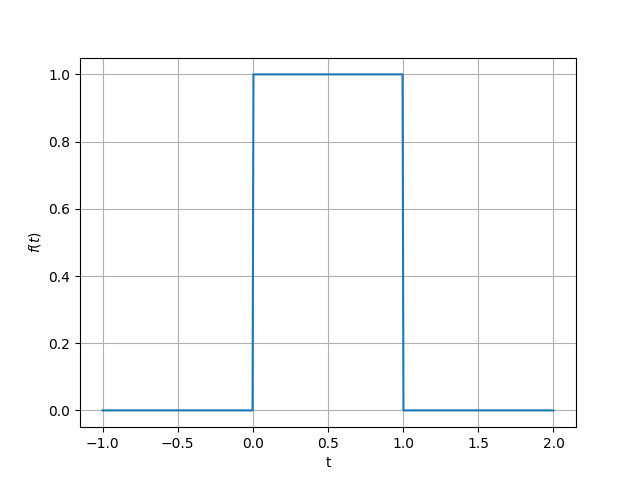
\includegraphics[width=\columnwidth]{f(t)_plot.png}
    \caption{Plot of f(t)}
    \label{plot}
\end{figure}
\begin{figure}[!ht]
    \centering
    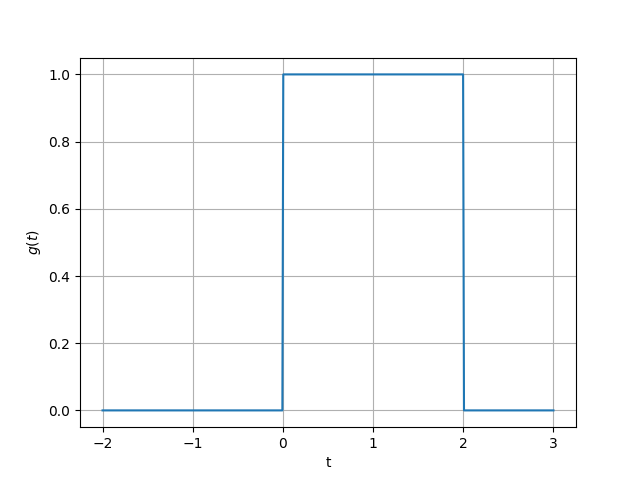
\includegraphics[width=\columnwidth]{g(t)_plot.png}
    \caption{Plot of g(t)}
    \label{plot}
\end{figure}
\begin{figure}[!ht]
    \centering
    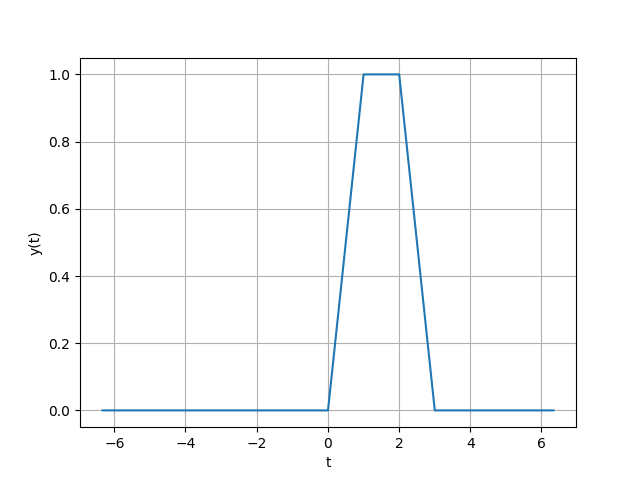
\includegraphics[width=\columnwidth]{y(t)_plot.png}
    \caption{Simulated plot of output signal y(t)}
    \label{plot}
\end{figure}
\end{document}
